\documentclass[a4paper,11pt]{article}
\usepackage{fullpage}
\usepackage{graphicx}
\usepackage{eqnarray,amsmath}


\pdfinfo{
/Title (ELEN3007-Assignment-2024)
/Author (Kgadile "Naar-Kie" Masemola)
/CreationDate (D:202303151636)
/ModDate (D:202409040530)
/Subject (ELEN3XXX Paper Format, 2024)
%/Keywords (ELEN3009, paper, project)
}

\title{ELEN3007A Group \underline{21} - Assignment 2024: \\ 
\large \emph{Application of Bayes’ Theorem for Locating a Robot’s
Position in an Enclosed Area}}
\author{Kgadile E Masemola (876729),  Thembinkosi Dhlamini (1234567),
 \\Siphokuhle Zulu (7654321), Lesego Gaborone (2176543)}
\date{September 13, 2024}

\begin{document}
\maketitle

\section*{Introduction and Background}
The assignment consideres that the position of $\beta$ is known, and after recording \emph{N} flashes at positions $x_k$, and inferes or answers the question: \emph{where is the robot}?\\
The azimuth angles at which the flashes are emmited, at random intervals, are quantified by $\theta_k$ which is uniformly distributed distributed. Since $\theta_k$ is uniformly distributed, we expect more recordings of $x_k$ near or around $\alpha$ which displays the vertical position underwhich the robot is expected to be. The mean value of $x_k$ is distance away from the assumed value of $\alpha$.

\subsection*{Assignment Criterion}
\begin{itemize}
	\item Geometry setup of the problem
		\begin{figure}[h]
        		\centering
        		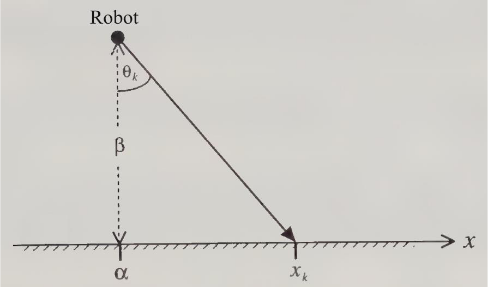
\includegraphics[scale=0.5]{elen3007assignfig.png} 
        		\caption{Geometry setup of the problem}
        \end{figure}
	\item $\theta_k$ assumed to be uniform, azimuth angles lying between $-\frac{\pi}{2}$ and $\frac{\pi}{2}$, it has the PDF:
		\begin{equation}
			p(\theta_k | \alpha, \beta, B) = f_{\Theta | \Omega, \beta, B}( \theta |\alpha) = \frac{1}{\pi}
		\end{equation}
	\item In order to relate the readings of $x_k$ to $\theta_k$, using elementary trigonometry, the derived expression is
		\begin{equation}
			\beta tan \theta_k = x_k - \alpha
		\end{equation}
	\item $x_k$ is independent and identically distributed from normal distribution.
\end{itemize}

\section*{Equations and Notations}
\begin{eqnarray}
	p(\theta_k | \alpha, \beta, B) = f_{\Theta | \Omega, \beta, B}(\theta)\\
	p(x_k |\alpha, \beta, B) = f_{X | \Omega, \beta, B}(x_k | \Omega = \alpha, \beta = b )
\end{eqnarray}

\section*{Assignment Answers}
\begin{enumerate}
  \item The given setup of the problem assumes that the photodetectors are placed on the x-axis above which the robot is located. Therefore, the signal comes from one side of the axis. This thus limits the range of the detectors to be within the range of $\pi$ (that is $-\frac{\pi}{2}$ to $\frac{\pi}{2}$). 
  \item 
  \item Etc.
\end{enumerate}

\section*{Conclusion}

\newpage
\appendix

\section{? Understanding the Assignment}
\begin{itemize}
	\item since we can't observe $\theta$, we transform to $x_k$. so that means we transform and drop the random variable $\Theta = \theta_k \Rightarrow X = x_k$  and it's PDF(\emph{prior}?) $p(\theta_k | \alpha, \beta, B)$ (given) to $p(x_k | \alpha, \beta, B)$ (proved)
	\item is $\alpha$ supposed to be assumed? if, then $\alpha$ is a constant and we want to find how far off we are from it as given by the measurements (observed data points)
	\item So, the $\alpha$ and $\beta$ are supposed to have a joint distribution right? and so after we observe $\beta = b$, we condistion $\alpha$ that is $p_{\alpha = a | \beta = b}$. But we are also given data whhich is $\{x_k\}^N _{k = 1}$ to infere the robot's position expressed by the posterior PDF $p_{\alpha | \{x_k\}^N _{k = 1}}(\alpha = a)$
\end{itemize}

\section{? Questions}
	\begin{enumerate}

		\item is this the marginal PDF? $p(\theta_k | \alpha, \beta, B) = \frac{1}{\pi}$
		\item is this the conditional distribution? $p(x_k | \alpha, \beta, B) = \frac{\beta}{\pi (\beta^2 + (x_k - \alpha)^2)}$
		\item in order to plot $p(\alpha | x_k, \beta, B)$, should we assume our own values for the parameters $\alpha$ and $\beta$?
		\item is this notation correct? $ p(x_k | \alpha, \beta, B) = f_{X | \Omega, \beta, B}(x_k | \alpha, \beta = b)$, where $b = constant$
		\item if then is posterior notation? $p(\alpha | x_k, \beta, B) = f_{\Omega | X, \beta, B}(\alpha) = \frac{\beta}{\pi (\beta^2 + (x_k - \alpha)^2)} \times \aleph$, where $\aleph$ is a \emph{proportional constant} of bayes transformation to posterior PDF
		\item and is? $p(\alpha | \{x_k\}^N _{k = 1}, \beta, B) = f_{\Omega | X, \beta, B}(\alpha | x_1,...,x_n, \beta = b ) = \prod^N _{k = 1} \frac{\beta}{\pi (\beta^2 + (x_k - \alpha)^2)} \times \aleph $
		\item is the $x$-position a matter of how far from the normal(that is $\alpha = 0 = x_0 = 0$ to $x_k = \mu_x$? is this the meaningful conclusion?
		\item because accordring to question 7, it says estimate $x$-position using 30 measurements. what are the other extra data points for? demo?  
		\item is this professional style report clear? and what is meant by effective data representation(graphs of distro. with different no. of N)? \emph{because} is (sub-\&)heading numbering necessary?		
		\item what does the demonstration require? effect of \emph{different number}(N) of observed data points?
		
	\end{enumerate}
	
\section{? other Questions}
	\begin{enumerate}
		\item do we need to apply maximum likelyhood solutions for the mean of data?
		\item if (or not) then the goal is to estimate the posterior mean? which can be given by a compromise between the prior mean $\mu_0$ and the maximum likelihood solution $\mu_{ML}$?
	\end{enumerate}


\end{document}